%  ClockGating.tex
%  Document created by seblovett on seblovett-Ubuntu
%  Date created: Sat 22 Feb 2014 13:20:20 GMT
%  <+Last Edited: Sun 23 Feb 2014 16:15:11 GMT by seblovett on seblovett-Ubuntu +>

\section{Clock Gating}

\subsection{Theory}

The clock in a sequential circuit can contribute 15-45\% of the power \cite{pedram1996power}.
Therefore it is a large area of potential power saving.
Clock gating is an approach of controlling the clock to individual modules of a design by either stopping or slowing down the clock with respect to a master clock \cite{841927}. 
An approach, seen in \cite{tellez1995activity}, involves stopping the clock to unused modules.

This method can be realised using two simple circuits seen in figures \ref{fig:cg:circuit1} and \ref{fig:cg:circuit2}.
Although figure \ref{fig:cg:circuit1} is functionally complete, in reality, a latch is needed to remove any glitches in the circuit.
These are fundamentally different to load-enable registers, where the input is multiplexed between the current value or the input.
The load-enable registers are still clocked at the master clock frequency.

\begin{figure}
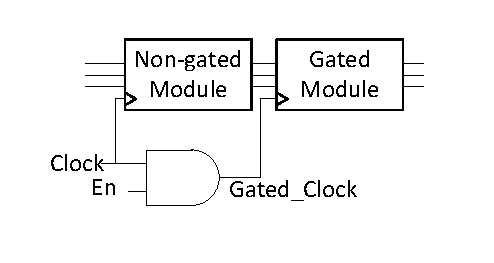
\includegraphics{Figures/clockgating_and.pdf}
\caption{Clock gating circuit using an AND gate}
\label{fig:cg:circuit1}
\end{figure}

\begin{figure}
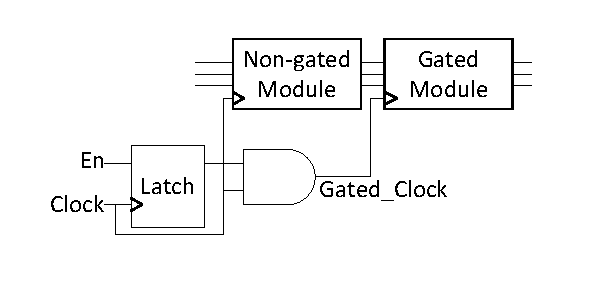
\includegraphics{Figures/clockgating_latch.pdf}
\caption{Clock gating circuit using an AND gate and a latch}
\label{fig:cg:circuit2}
\end{figure}

\subsection{Synthesis Techniques}

A gating function is typically defined by the designer within the RTL design stage.
However, a more common approach is to allow the synthesis tool to obtain the gating functions from a gate-level netlist \cite{benini1999symbolic, hurst2008automatic}.

The general outline for the synthesis is to find the clock gating function for each flip-flop.
The flip-flops are then grouped so that they are driven by the same function. 
The problem of simplifying the gating function is looked at in \cite{han2012synthesis}. 
Here, an algorithm is suggested where the gating function is shared by existing combinational logic.
This was shown to reduce the logic added by introducing clock gating.

\subsection{Advantages}

Good things about using this.

\subsection{Disadvantages}

Bad things about using this.







